\chapter{STATE OF THE ART}
\label{see:art}

% Hier werden zwei wesentliche Aufgaben erledigt:

% 1. Der Leser muß alles beigebracht bekommen, was er zum Verständnis
% der späteren Kapitel braucht. Insbesondere sind in unserem Fach die
% Systemvoraussetzungen zu klären, die man später benutzt. Zulässig ist
% auch, daß man hier auf Tutorials oder Ähnliches verweist, die hier auf
% dem Netz zugänglich sind.

% 2. Es muß klar werden, was anderswo zu diesem Problem gearbeitet
% wird. Insbesondere sollen natürlich die Lücken der anderen klar
% werden. Warum ist die eigene Arbeit, der eigene Ansatz wichtig, um
% hier den Stand der Technik weiterzubringen? Dieses Kapitel wird von
% vielen Lesern übergangen (nicht aber vom Gutachter ;-), auch später
% bei Veröffentlichungen ist "Related Work" eine wichtige Sache.

% Viele Leser stellen dann später fest, daß sie einige der Grundlagen
% doch brauchen und blättern zurück. Deshalb ist es gut,
% Rückwärtsverweise in späteren Kapiteln zu haben, und zwar so, daß man
% die Abschnitte, auf die verwiesen wird, auch für sich lesen
% kann. Diese Kapitel kann relativ lang werden, je größer der Kontext
% der Arbeit, desto länger. Es lohnt sich auch! Den Text kann man unter
% Umständen wiederverwenden, indem man ihn als "Tutorial" zu einem
% Gebiet auch dem Netz zugänglich macht.

% Dadurch gewinnt man manchmal wertvolle Hinweise von Kollegen. Dieses
% Kapitel wird in der Regel zuerst geschrieben und ist das Einfachste
% (oder das Schwerste weil erste).

%\ldots state of the art \ldots

%\todo{write state}

This chapter first discusses the effort to minimize the \acrshort{TCB} of virtual machines and then delves into the mechanisms for securely orchestrating containers in cloud environments. In particular, security orchestration refers to how containers can be deployed, operated, and managed securely in untrusted cloud environments.


\section{Minimizing the VM's TCB}

Reducing the size (\acrshort{TCB}) of a VM can enhance its performance, resulting in fast boot time and reduced memory consumption. Consequently, various research groups have conducted extensive studies throughout the last decade. The proposed solutions encompass unikernel~\cite*{10.1145/2499368.2451167}, application kernel~\cite*{gvisor, quark}, 
and the tailoring of the full-stack guest kernel~\cite*{Kata-Containers, tiny_linux}, etc.


Unikernel~\cite*{10.1145/2499368.2451167} uses a single-purpose, statically sealed, minimalist LibOS virtual machine to run individual programs. This single-purpose virtual machine, also known as an appliance, contains only the code and data the application needs. At compile time, the unikernel 
encapsulates the application 
binary and the required LibOS modules into an image that can be run directly on a virtual machine manager (VMM). At runtime, the appliance provides only the application's required services and utilizes the \acrshort{VMM} for isolation and resource multiplexing. Compared to traditional virtual machines (based on rich operating systems 
such as Linux), the LibOS in an appliance is smaller. Thus, it boots faster and has a smaller memory footprint while maintaining the same isolation level. Furthermore, the unikernel's \acrshort{TCB} is typically smaller than a container, picoproces, and traditional virtual machine~\cite*{10.1145/3436512}. Also, the appliance 
employs the VM ABI to communicate with the host. It is much smaller than the system call API and, therefore, easier to protect~\cite*{10.1145/3436512}. However, the lack of support for dynamic code loading, process abstraction, and debug tools limits its flexibility~\cite*{10.1145/3436512, 10.1145/3267809.3267845}.


Kylinx~\cite*{10.1145/3436512} exemplifies the concept of \acrshort{pVM}, which uses \acrshort{VMM} as the operating system and appliances as processes. It extends unikernel to provide process-level abstraction and dynamic library loading. The above two features are realized by dynamic mapping at the page level and library level. 
Specifically, at the page level, it supports \acrshort{pVM} fork and \acrshort{pVM}-to-\acrshort{pVM} communication. A \acrshort{pVM} can use the fork interface and the VMM's memory-sharing mechanism to generate a new \acrshort{pVM}. The communication between the two is enabled by an event channel and shared pages. At the library level, 
Kylinx can load shared libraries into the appliance at runtime by adding a dynamic segment to the appliance's original memory layout. This allows the \acrshort{pVM} to perform online library updates. With the above approach, Kylinx retains the benefits of unikernel and improves its flexibility, efficiency, and applicability.

 
\begin{figure}[htp]
    \centering
    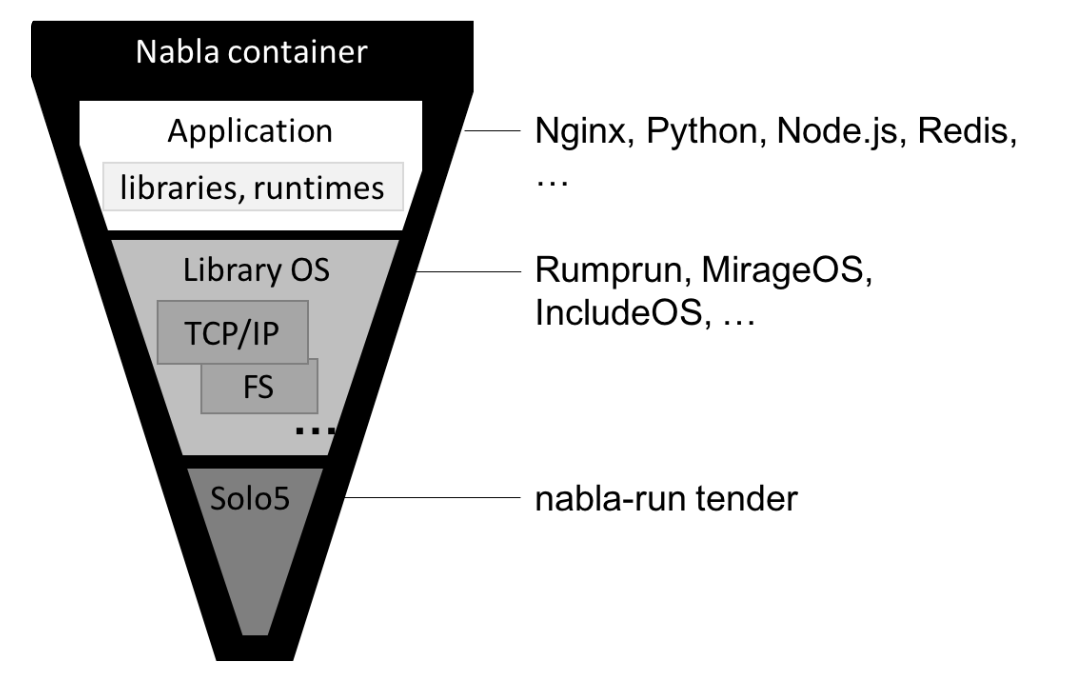
\includegraphics[width=0.4\textwidth]{images/nabla.png}
    \caption[IBM nabla architecture]{IBM nabla architecture (from~\cite*{Nabla})}
    \label{fig:nabla}
\end{figure}

IBM Nabla~\cite*{10.1145/3267809.3267845} proposes a novel secure container model, namely single-container- per- unikernel VM. It runs unikernel VMs as processes, increasing flexibility while maintaining performance and security. Figure~\ref{fig:nabla} shows the architecture of IBM Nabla, which consists of a Tender and a unikernel VM. Tender is a \acrshort{VMM} 
responsible for managing unikernel VMs. In particular, the unikernel VM accesses Tender using procedure calls instead of hyper calls. To provide the same level of isolation to unikernel VMs as provided by hardware virtualization, Tender runs in Seccomp mode. By default, Tender's Seccomp whitelist includes only seven system calls. Therefore, the unikernel VM cannot 
force Tender to execute system calls outside the whitelist. In addition, Tender runs the unikernel VM as a process. Specifically, Tender as a host process dynamically loads the unikernel image into its address space. It then configures the Seccomp filter and starts the unikernel VM by jumping into the unikernel's code entry point. Once started, the unikernel uses 
the Tender's registers and stack and accesses the services provided by the Tender through the function call. In summary, unikernel as a process eliminates the need for virtualized hardware, can be debugged and managed using standard process tooling, and improves performance by avoiding hypercalls.

% Quark~\cite*{quark} provides a pVM-like architecture. They both support dynamic shared library loading and use a minimalist guest kernel. However, Quark differs from Kylinx in several ways. First, Quark does not currently support pVM fork and pVM inter-process communication. Second, unlike the Kylinx architecture, 
% where the VMM can run multiple appliances, the VMM in Quark only supports running one guest. Furthermore, the guest kernel in Quark is more like a forwarding kernel. It implements a small number of system calls and forwards others to the host. In addition, Quark's guest kernel implements process 
% management and memory management. This allows Quark guests to run multiple processes. More details about Quark can be found in Section~\ref{sec:Quark}.

Researchers have also made efforts to minimize the size of the full-stack guest kernel. For instance, Kata containers~\cite*{Kata-Containers} utilize a highly optimized QEMU and guest Linux kernel to create a virtual machine for container execution. The guest Linux kernel includes only the necessary modules for running the containers. 
A detailed explanation of the Kata containers can be found in Section~\ref{sec:Kata}. Additionally, Tiny Core Linux~\cite*{tiny_linux} aims to minimize the size of the Linux kernel by trimming off unused modules. Therefore, VMs utilizing Tiny Core Linux as the guest kernel exhibit improved performance and smaller \acrshort{TCB} than those running vanilla Linux distributions.


Quark~\cite*{quark} and gvisor~\cite*{gvisor}, similar to Kata containers, operate containers within virtual machines. However, their guest kernel is an application kernel, which implements a small number of system calls and forwards others to the host. Due to its reliance on the host for most of its functionality, the guest kernel is notably simplified. Quark also introduces a pVM-like 
architecture. Both Quark and Kylinx support dynamic shared library loading. Nevertheless, Quark's guest kernel goes beyond Kylinx by incorporating process and memory management functionalities. This allows a Quark guest to run multiple processes. For more details about Quark, please refer to Section~\ref{sec:Quark}.


\section{Secure Orchestration}
Since the introduction of Container-as-a-Service, securely deploying, manipulating, and managing containers in untrusted cloud environments has been troubling tenants. To this end, a range of solutions for the orchestration of containers securely is proposed. These solutions aim to automate the deployment and management of containers using container orchestration platforms such as Kubernetes while ensuring the 
confidentiality and integrity of tenants' private and sensitive data in cloud environments. This section describes three mechanisms for securely orchestrating containers.

Pama~\cite*{Johnson2023ParmaCC} offers a mechanism for securely running a pod (a set of containers) in AMD SEV-SNP~\cite*{SEV_SNP_white_book} using a so-called execution policy. It supports remote attestation and secret provisioning and implements two types of confidential filesystems, i.e., integrity-protected and encrypted filesystems. These filesystems protect the container root filesystem 
(consisting of the container image layers and scratch space) and the user's sensitive data. Each container image layer (pulled by the Containerd~\cite*{containerd} and stored in a host-side block device) is mounted by Pama as an 
integrity-protected read-only guest file system. When accessing the file system, a guest filesystem driver uses reference values in the execution policy to force integrity checks. This way, Pama ensures the host cannot tamper with the container image.
On the other hand, encrypted filesystems protect block devices and volumes containing users' private sensitive data. When an encrypted file system is accessed, a guest driver decrypts the corresponding memory-mapped block and copies the output to the guest's private memory. 
\begin{figure}[htp]
    \centering
    \begin{subfigure}[b]{0.45\textwidth}
        \centering
        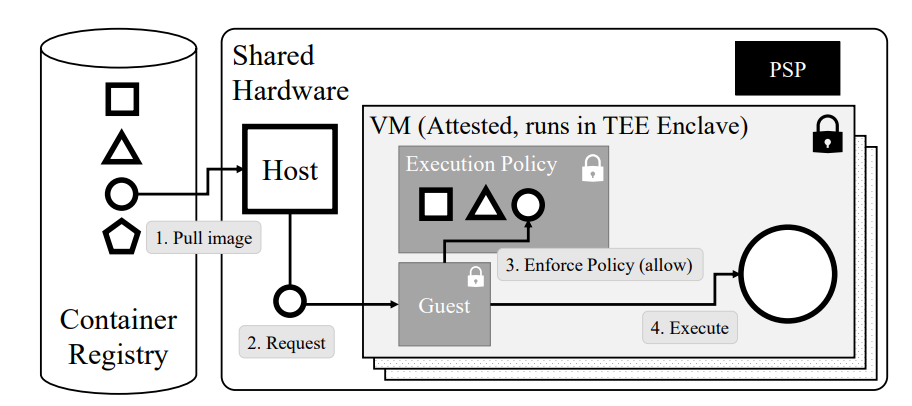
\includegraphics[width=\textwidth]{images/pama_policy.png}
        \caption{Execution policy}
        \label{fig:pama_policy}
    \end{subfigure}
    \hfill
    \begin{subfigure}[b]{0.45\textwidth}
        \centering
        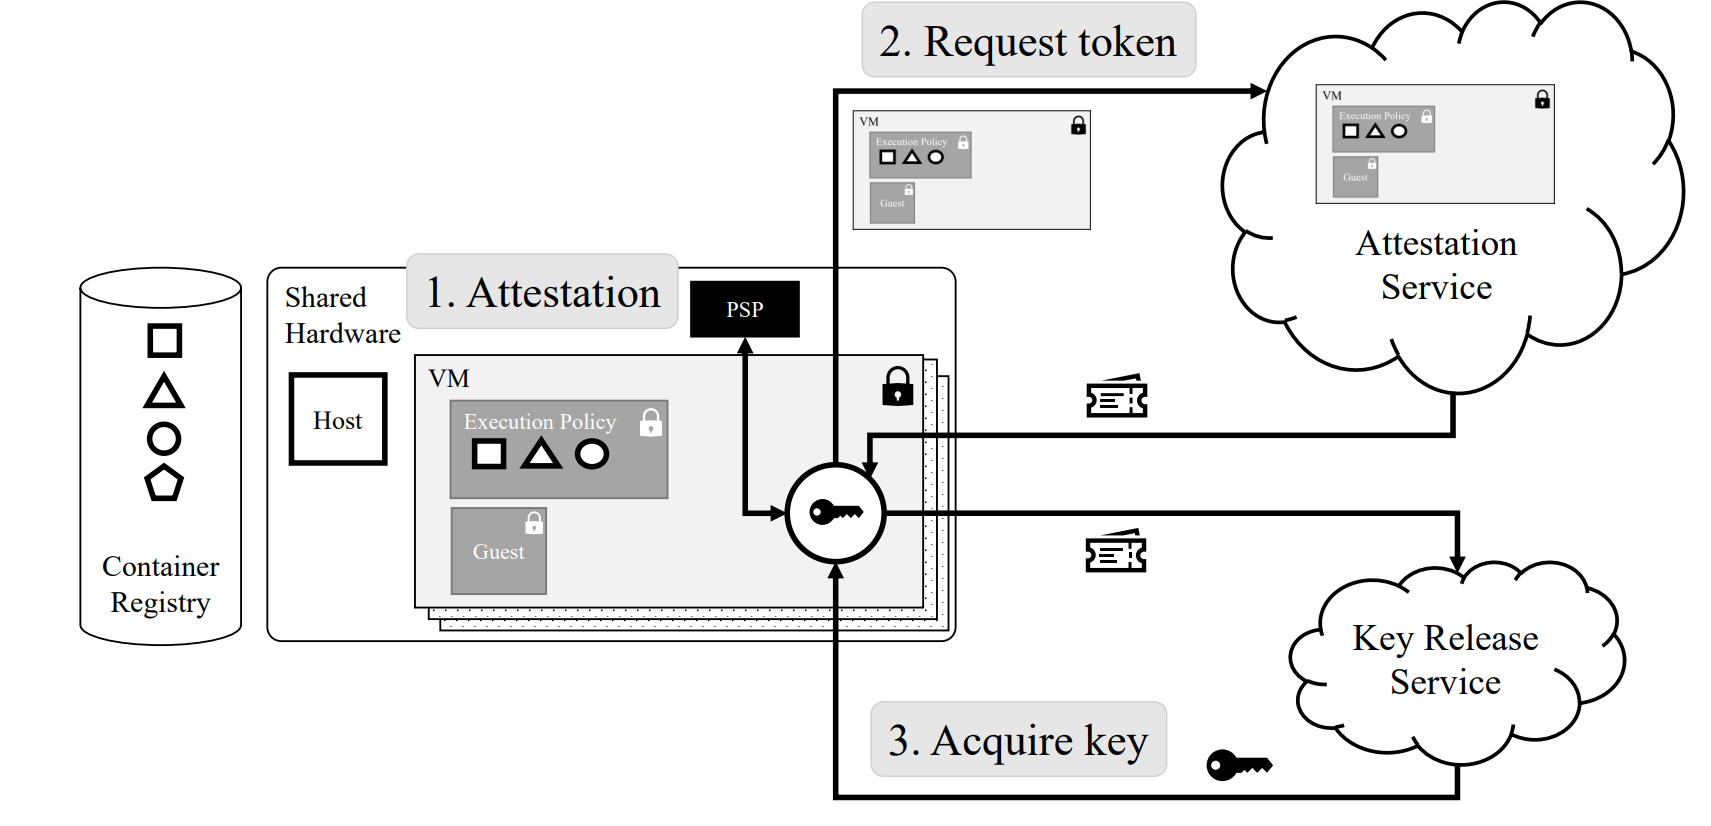
\includegraphics[width=\textwidth]{images/pama_atte.png}
        \caption{Attestation workflow}
        \label{fig:pama_atte}
    \end{subfigure}
    \hfill
       \caption[The execution policy and attestation workflow of Pama]{The execution policy and attestation workflow of Pama (figures from~\cite*{Johnson2023ParmaCC} )}
       \label{fig:pama}
\end{figure}

For secure orchestration, Pama provides the guest with an attested execution policy. It is passed to the guest during initialization and attested by the relying party. This policy is defined by the guest owner and describes the operations that the host is allowed to perform when orchestrating 
containers. The guest agent, responsible for communicating with the host, can decide whether to execute commands based on this policy (Figure~\ref{fig:pama_policy}).  


In Pama, users' sensitive data is transmitted to the guest in an encrypted manner while its encryption key is uploaded to the key release service. In order to decrypt the data, the guest needs to perform remote attestation. The flow of remote attestation and provisioning 
is shown in Figure~\ref{fig:pama_atte}. Guest first requests an attestation report containing the hash of an RSA public key from the AMD PSP~\cite*{snp_firmware}. It then sends the report and the public key to the attestation service. After verifying the identity of the guest, 
the attestation service issues an attestation token for it. With this token, the guest can obtain a key cryptographically protected by the public key from the key release service.

 
\begin{figure}[htp]
    \centering
    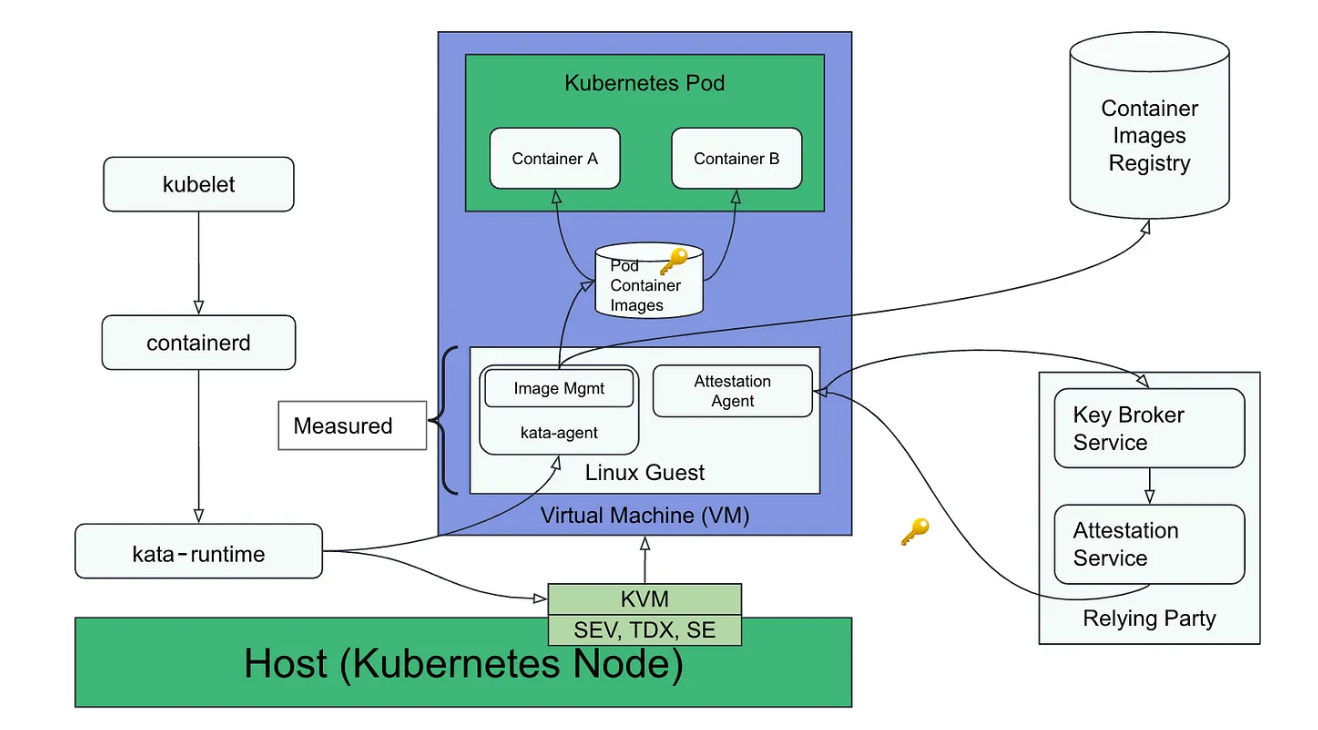
\includegraphics[width=0.6\textwidth]{images/confidentail_kata.png}
    \caption[Overview of confidential container]{Overview of confidential container (from ~\cite*{confidential_kata})}
    \label{fig:confidentail_kata}
\end{figure}

The confidential container~\cite*{confidential_kata} is another solution that protects users' sensitive data at the pod level. It originates from the Kata container~\cite*{Kata-Containers} and uses \acrshort{TEE} to provide privacy for the data and code inside a pod. Figure~\ref{fig:confidentail_kata} presents its architecture, i.e., a Kubernetes pod runs in a 
TEE-protected virtual machine. In order to prevent the host from tampering with the container's image, the confidential container offloads the image management from the Containerd\cite*{containerd} to the Image Mgmt module within the guest. It is responsible for image pulling, unpacking, and generating the 
application bundle. Since untrusted third parties manage container images, all container images are either encrypted or signed. Note that image encryption only occurs if the image contains sensitive data or code. Upon receiving the image, the guest must perforce image decryption and signature 
verification using a key managed by the relying party. In this case, the attestation agent uses the KBS attestation protocol~\cite*{kbs_Attestation_protocol} to prove its identity to the relying party and retrieve the corresponding key. An explanation of the KBS attestation protocol can be found in Section~\ref{sec:kbs}. The unpacked images are saved in 
the TEE-protected VM memory and used to create containers. The untrustworthy kata runtime sends commands to the kata agent inside the guest for container 
orchestration. For security reasons, like Pama, the confidential container allows the user to define a policy for the Kata agent~\cite*{kata_api_restriction}. This policy is a blacklist that describes the commands that the Kata agent will reject. Currently, the project does not support persistent trusted storage. 
Some discussion about it can be found in~\cite*{confidentail_kata_storage}.

\begin{figure}[htp]
    \centering
    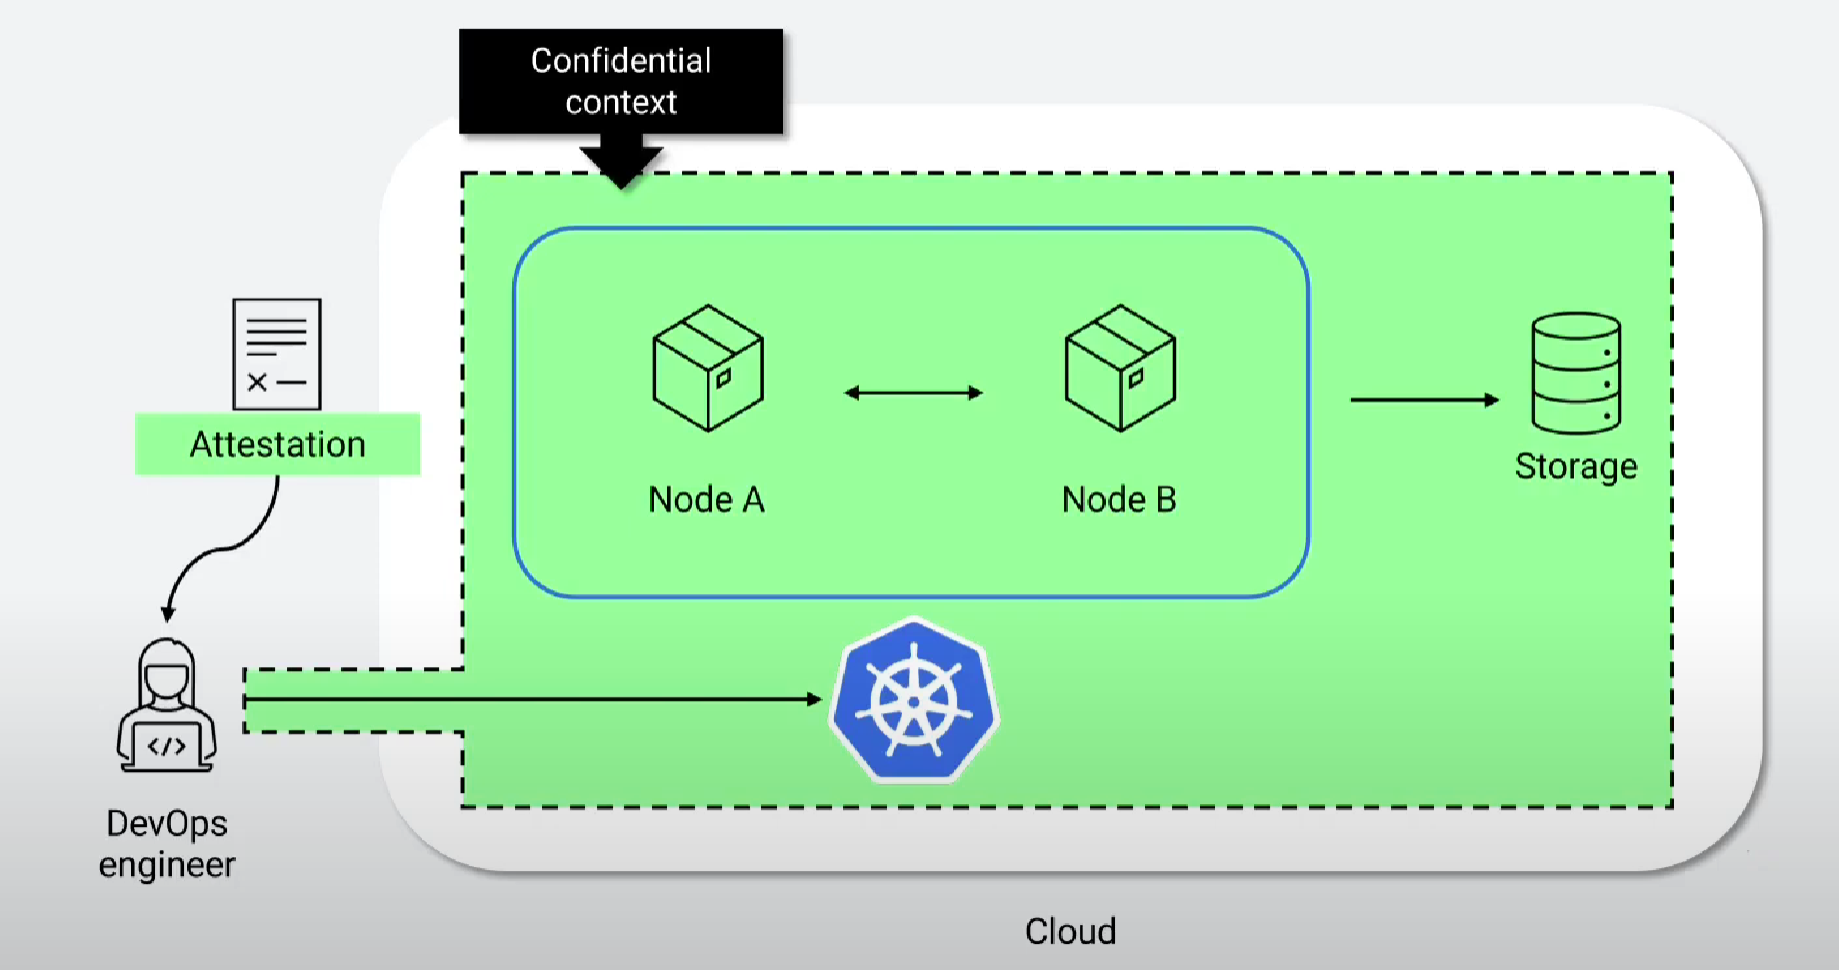
\includegraphics[width=0.6\textwidth]{images/constellation_arch.png}
    \caption[Overview of constellation]{Overview of constellation (from~\cite*{Constellation_Always_encrypted})}
    \label{fig:constellation_arch}
\end{figure}

Constellation~\cite*{Constellation}, as shown in Figure~\ref{fig:constellation_arch}, is a solution for confidential Kubernetes at the node level. It runs Kubernetes nodes in confidential VMs and provides a lift-and-shift way to run workloads in a verifiable and isolated cluster. The verifiability and isolation are achieved through node-to-node mTLS, 
node-to-node attestation, cluster-to-client attestation, and storage encryption~\cite*{Constellation_Encrypted_Kubernetes}. To this end, the sensitive data in the cluster are protected at rest, in transit, and in use. 
 


Constellation enables the cluster to scale securely according to the user's policy, and the whole cluster can consistently be attested in a transitive way. The workflow is shown in Figure~\ref{fig:constellation_join}. The client verifies the first node in the cluster using remote attestation and TLS. 
Once verified, the client provides a configuration file to the node to bootstrap Kubernetes and initialize all constellation components. This node then returns a Kubeconfig to the user over the TLS channel. Since the Kubeconfig is only accessible to the cluster owner, the cloud provider or other tenants 
cannot reach the cluster. Instead of verifying every new node by hand, the constellation provides a service called Join Sevice. It runs on the master node and verifies the new node before it joins the cluster using remote attestation.
\begin{figure}[htp]
    \centering
    \begin{subfigure}[b]{0.45\textwidth}
        \centering
        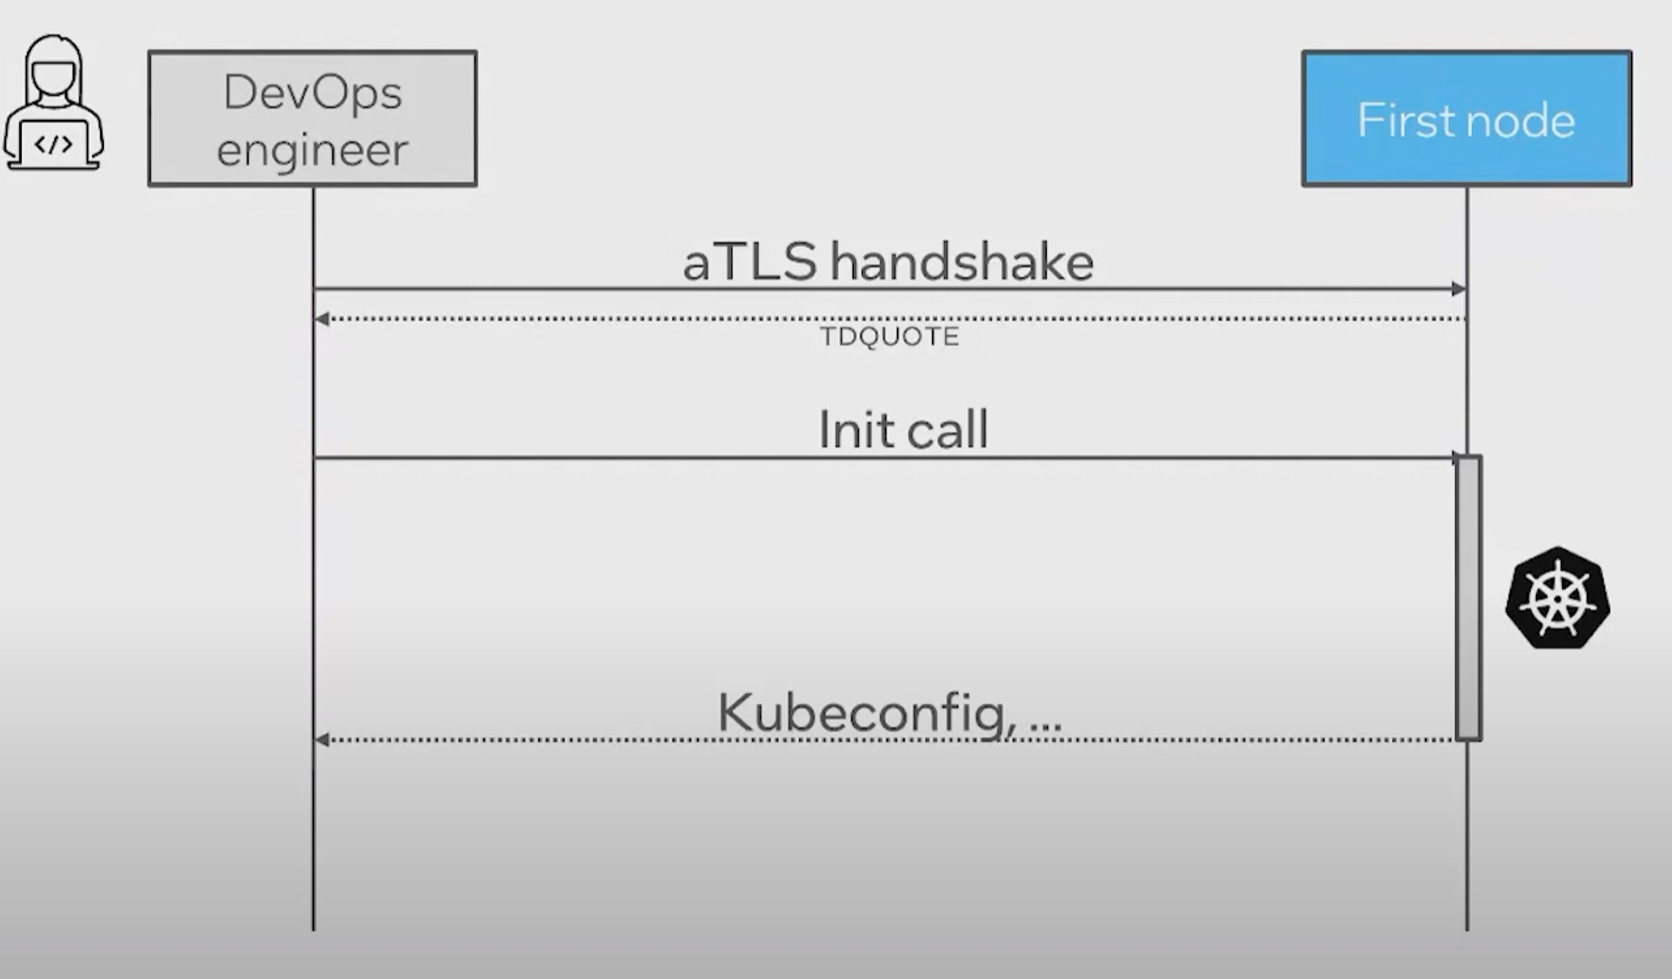
\includegraphics[width=\textwidth]{images/constellation_join_1.png}
        \caption{Cluster initialization}
        \label{fig:constellation_join_1}
    \end{subfigure}
    \hfill
    \begin{subfigure}[b]{0.45\textwidth}
        \centering
        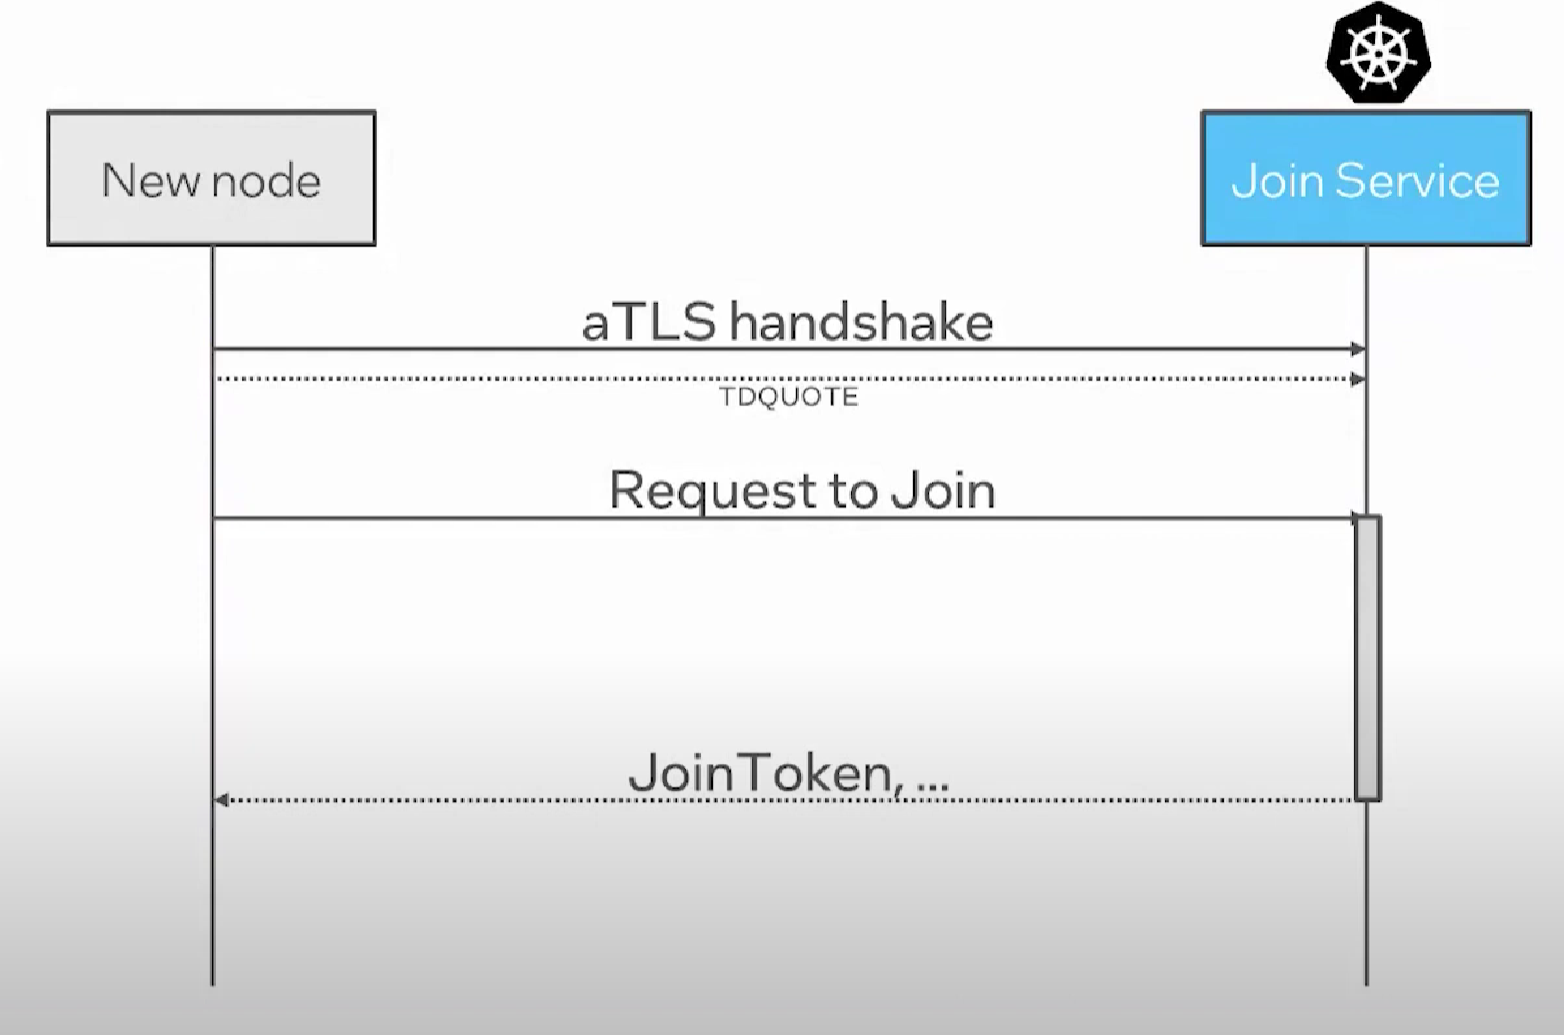
\includegraphics[width=\textwidth]{images/constellation_join_2.png}
        \caption{Workflow for autonomous join}
        \label{fig:constellation_join_2}
    \end{subfigure}
    \hfill
       \caption[Constellation's JoinService]{Constellation's JoinService (Figures from~\cite*{Constellation_Always_encrypted})}
       \label{fig:constellation_join}
\end{figure}

Constellation protects workloads within the cluster from infrastructure-based threats. This includes compromised cloud provider admin exploits, etc. Since all cluster nodes, including the master node running the control plane, are trusted, workloads in the cluster can be safely orchestrated. 
Furthermore, the secrets are provisioned by the cluster owner and managed by Kubernetes. An attacker cannot steal the cluster-managed secrets because the cluster is fully isolated.
 
 
Among the three mentioned solutions, Constellation~\cite*{Constellation} has the largest \acrshort{TCB} since it put the entire cluster under the protection of \acrshort{CVM}s。 Consequently, it also inherits a larger attack surface. Additionally, Both Pama~\cite*{Johnson2023ParmaCC} and confidential container~\cite*{confidential_kata} use a dedicated 
guest kernel (e.g., Linux) and therefore have larger \acrshort{TCB}s than pVM and process-based TEE solutions, such as Scone~\cite*{10.5555/3026877.3026930}. Nevertheless, Pod-level solutions (e.g., Pama and confidential container) have a smaller security boundary compared to Scone due to Scone's utilization of the system 
call API as its security boundary. In contrast, Pod-level solutions use the VM-ABI as the secure boundary, e.g., Hypercall. Finally, the confidential container necessitates using a modified Containerd~\cite*{containerd}, thereby imposing an additional burden on the configuration of its environment.



\cleardoublepage

